\documentclass[tikz]{standalone}
\usepackage{tikz}
\begin{document}
\begin{figure}
\centering
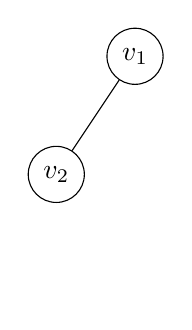
\begin{tikzpicture}[main/.style = {draw, circle, fill=white}]
  \node[main] (1) {$v_{1}$};
  \node[node distance={15mm}] (1111111111111111111111111111111111111111111111111111111111111111111111111111111111111111111111111111) [below of=1] {};
  \node[node distance={10mm}, main] (2) [left of=1111111111111111111111111111111111111111111111111111111111111111111111111111111111111111111111111111] {$v_{2}$};
  \draw (1) -- node[left] {} (2);
  \node[node distance={15mm}] (2222222222222222222222222222222222222222222222222222222222222222222222222222222222222222222222222222) [below of=2] {};
\end{tikzpicture}
\end{figure}
\end{document}
